%%%%%%%%%%%%%%%%%%%%%%%%%%%%%%%%%%%%%%%%%%%%%%%%%%%%%%%%%%%
\chapter{The Standard Model of Particle Physics}%%%%%%%%%%%%%%%%%%%%%%%%%%%%%%%%%%%%
%%%%%%%%%%%%%%%%%%%%%%%%%%%%%%%%%%%%%%%%%%%%%%%%%%%%%%%%%%%
\label{ch:SM_intro}
The Standard Model of particle physics has been hugely successful in explaining what our universe consists of at the smallest length scales, and how these constituents interact with each other. It recieved a final, spectacular confirmation in 2012, when a Higgs boson consistent with the predictions of the Standard Model was discovered by the CMS and ATLAS experiments at CERN. It is well known, however, that the Standard Model is incomplete as a description of our universe, for instance since it gives no explanation for dark matter. There are also more technincal problems with the Standard Model, such as the hierarchy problem of the Higgs boson mass loop corrections and the arbitrariness of the model parameters.

The present chapter gives an introduction to the principles that underlie the construction of the Standard Model, and outlines the derivation of the model. The presentation is based on \cite{Mandl-Shaw} and \cite{Peskin-Schroeder}.

\section{Symmetries and conservation laws}
Symmetries are manifest in many physical systems. For instance, the special theory of relativity is symmetric under boosts and rotations, as well as translations in space and time. There is a deep relationship between symmetries and the conservation of physical quantities. This result is known as Noether's theorem, and was proven by Emmy Noether in 1915. It states that {\it every differentiable symmetry of the action of a physical system has a corresponding conservation law}. In the example of special relativity, the symmetries under translations in time and space correspond to conservation of energy and momentum.%, and the symmetry under rotation corresponds to conservation of angular momentum. \marginpar{What is the conserved quantity under boosts? Is it that ljyubliajsnski polarization vector? Check.}

\subsection{Description by groups}
It is often convenient to describe the symmetries of physical systems in the language of group theory. A group is a set of objects which are closed under some binary operation -- meaning that any combination of two group elements yield another group element. The set of all Lorentz boosts and rotations in special relativity form a group, called the Lorentz group, and together with all spatial translations they form the Poincar\'{e} group. 

The experimental fact that there exist a number of conserved quantities in particle physical systems -- examples include energy and momentum, but also electrical and colour charge, among others -- can be used to construct a theory of particle interactions, by finding the symmetries, and the symmetry groups, that correspond to these quantities and demanding that the theory be symmetric under their action.

\section{The Standard Model of Particle Physics}

\subsection{Phenomenology of the Standard Model}
The Standard Model consists of 12 fermions with corresponding antifermions, a number of vector gauge bosons and one scalar boson. The gauge bosons mediate interactions between the particles. There are three fundamental interactions in the Standard Model: The electromagnetic interaction, the weak interaction and the strong interaction. Not all particles couple to each other with all of the interactions. 

The fermions are divided into two groups, the quarks and leptons. There are six different {\it flavours} of quarks, called up, down, strange, charm, bottom and top, in order of increasing mass. They are subdivided into three generations of pairs, up/down, charm/strange and top/bottom. The up, charm and top quarks carry quanta of +2/3 of the fundamental electrical charge $e$, while the down, strange and bottom quarks carry -1/3 $e$. There are also six leptons, of which three are charged. They are called electron, muon and tau. They belong in each their own generation, together with their neutral counterpart, the electron neutrino, muon neutrino and tau neutrino, respectively. 

The vector gauge bosons consist of the photon, the $Z$ and $W$ bosons and the gluon. The photon is the mediator of electromagnetic interactions, the $Z$ and $W$ mediate the weak interaction and the gluon mediates the strong interaction. The photon, $Z$ boson and gluon are all neutral, and they are their own antiparticles. The photon and gluon are massless, while the $W$ and $Z$ bosons are quite heavy. The $W$ carries one elementary unit of electric charge, and is thus distinct from its antiparticle, with a difference in sign for the particle and antiparticle states. The scalar boson of the Standard Model is the Higgs boson, which is responsible for giving particles their observed mass through the Higgs mechanism. It is electrically neutral and very massive.

Among the fermions, only the quarks couple to the strong interaction. All the fermions couple with the weak interaction, while only the electrically charged particles couple electromagnetically -- {\it i.e.}\ all except the neutrinos. They couple to the Higgs field proportionally to their mass, so that for instance the top quark, which is the heaviest Standard Model particle, couples the strongest, and the neutrinos, being very light, hardly couple at all. A schematic overview of the particles in the Standard Model is shown in fig.\ \ref{fig:SM_particles}.
\begin{figure}[hbt]
	\centering
	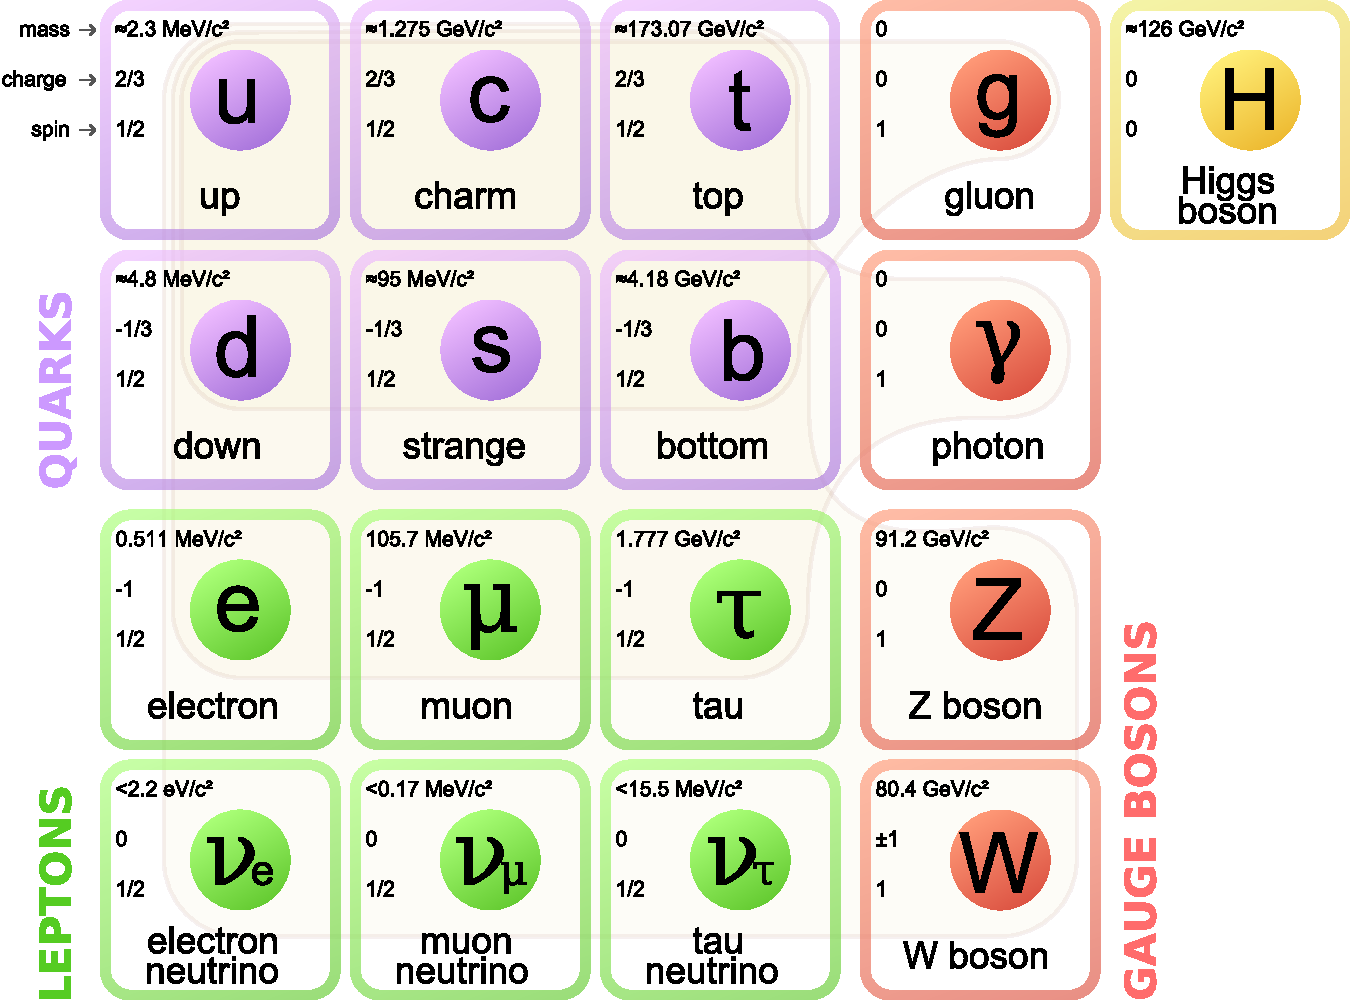
\includegraphics[width=0.8\textwidth]{figures/susyintro/Standard_Model_of_Elementary_Particles.pdf}
	\caption{An overview of the particles of the Standard Model and their interactions, from \cite{Wikimedia_SM_particles}.}
	\label{fig:SM_particles}
\end{figure}

The flavours of the quarks and leptons are conserved in the electromagnetic and strong interactions. For instance, a top quark cannot change into a charm or up quark by emission of a photon or gluon. The weak interaction enables the top quark to change into a bottom quark, or a tau lepton to change into a tau neutrino, through the emission of a charged $W$ boson. This would still seem to conserve the {\it generation} of quark or lepton, but breaking of generation is also made possible through the mechanism of {\it generation mixing}, quantified by the Cabibbo-Kobayashi-Maskawa (CKM) matrix for the case of quarks and the Pontecorvo-Maki-Nakagawa-Sakata (PMNS) matrix for the leptons. The PMNS mixing also explains the observed phenomenon of {\it neutrino oscillations}.

\subsection{Constructing the Lagrangian of the Standard Model}

The Standard Model is a quantum field theoretic model, and may be stated in terms of a Lagrangian density function $\mathcal{L}$. The guiding principle for constructing the Lagrangian is {\it gauge invariance}. Gauge degrees of freedom are physical degrees of freedom which are ``superflous'', in the sense that they do not have any observable consequences. An example is Maxwell's theory of electromagnetism, where the electromagnetic vector potential $A^\mu$ is undetermined up to the addition of a total derivative term $\partial^\mu \phi$. The gauge freedom is exploited by requiring that the Lagrangian, which determines the physical dynamics, does not change when the gauge degrees of freedom are varied, {\it i.e.}\ that it is gauge invariant. This invariance is related to conservation of physical quantities by Noether's theorem.

\subsection{The Lie groups of the Standard Model}

The Standard Model is based on gauge invariance under three Lie groups of quadratic matrices, the famous $U(1)_Y\times SU(2)_L\times SU(3)_C$. The number in the parenthesis gives the matrix dimension of the group. The symbols $S$ and $U$ stand for {\it special} and {\it unitary}, respectively. Unitary means that the matrices are unitary, and special means they have determinant 1. The groups are Lie groups, which means that they are continuous, and thus that any transformation of a group element may be constructed from infinitesimal transformations. The group elements, and the objects on which the group acts, may be given in several {\it representations}. In the case of matrix groups this means matrices and vectors of different dimension. For an $SU(n)$ group, the two most important representations are the {\it fundamental} representation, where the vectors have dimension $n$, and the {\it adjoint} representation, where the vectors have dimension $n^2-1$. In the Standard Model, the fermions transform in the fundamental representation, while the gauge bosons transform in the adjoint representation.

An element $G$ of an $SU(n)$ group may generally be written as\footnote{Here and in the following, repeated indices are summed over.} 
\begin{align}
	G = e^{i\alpha_a T_a},
\end{align}
where $T_a$ are the $n^2-1$ generators of the Lie algebra of the group. The generators themselves are in the fundamental representation represented by traceless complex $n\times n$ matrices -- for $SU(2)$, these are the Pauli matrices $\sigma_i$, and for $SU(3)$ they are the Gell-Mann matrices $\lambda_i$ -- and in the adjoint representation by the {\it structure coefficients} $f_{abc}$ as $(T_a)_{bc} = f_{abc}$. The structure coefficients are determined from the Lie algebra as
\begin{align}
	[T_a, T_b] = i f_{abc}T_c.
\end{align}

\subsection{Constructing a gauge theory}
The particle content of the Standard Model is input into the Lagrangian by inserting fermionic fields, {\it i.e.}\ Dirac spinor fields, and imposing the desired gauge invariance on these fields. The basic Dirac term, called the Dirac bilinear, for some spinor field $\psi$, is\footnote{We will, for what follows, set $\hbar = c = 1$.} 
\begin{align}
	\bar \psi (i\gamma^\mu \partial_\mu - m) \psi = \bar \psi (i\slashed\partial - m)\psi, \label{eq:diracbilinear}
\end{align}
where $\gamma_\mu$ are the Dirac matrices, $m$ is the mass of the spinor field, and $\bar\psi \equiv \psi^\dag \gamma_0$. Next, we impose gauge invariance. The group transformation of an $SU(n)$ group may be written in the fundamental representation as
\begin{align}
	G(x) = e^{ig\alpha_a(x)T^a},
\end{align}
where $\alpha(x)$ are $n$ arbitrary real differentiable functions and $T^a$ are the generators of $SU(n)$ in the fundamental representation. We assume that the Lagrangian consists of $n$ Dirac bilinear terms with fields $\psi_i$, and that they are put into an $n$-dimensional multiplet $\Psi = (\psi_1, \psi_2, ..., \psi_n)^T$ such that the basic Dirac Lagrangian reads
\begin{align}
	\mathcal{L}_0 = \bar\Psi(i\slashed\partial - m)\Psi
\end{align}
where we assume that all fields have the same mass $m$.\footnote{This assumption is often wrong in the case of the Standard Model, but finds its solution in the Higgs mechanism.} The group transformations of the multiplet and its adjoint are then 
\begin{align}
	\Psi(x) &\overset{G}{\to} e^{(ig\alpha_a(x)T^a)} \Psi(x),\\
	\bar\Psi(x) &\overset{G}{\to} \bar\Psi(x) e^{(-ig\alpha_a(x)T^a)}.\nonumber
\end{align}
If we apply these transformations to the basic Lagrangian, it becomes
\begin{align}
	\mathcal{L}_0 = &\bar\Psi(x)(i\slashed\partial - m)\Psi(x)\nonumber\\
	\overset{G}{\to} &\bar\Psi(x) e^{(-ig\alpha_a(x)T^a)}(i\slashed\partial - m)e^{(ig\alpha_a(x)T^a)} \Psi(x)\\
	=	&\bar\Psi(x)(i\slashed\partial - m)\Psi(x) - g\bar\Psi(x) T^a\slashed\partial \alpha^a(x) \Psi(x).\nonumber
\end{align}
Thus, the basic Dirac Lagrangian is not gauge invariant, since we have picked up an additional term. Gauge invariance may be achieved by adding a term of the form 
\begin{align}
	-\bar\Psi(x) ig\gamma^\mu \alpha_a(x)A^a_\mu(x) \Psi(x)\label{eq:covariantderivativeterm}
\end{align}
to the Lagrangian, where $A^a_\mu(x)$ is some new field, which we require to transform under $G$ as
\begin{align}
	A^a_\mu(x) \overset{G}{\to} A^a_\mu(x) + \partial_\mu \alpha^a(x).
\end{align}
If we apply $G$ to the sum of the Dirac bilinear with this new term, it is invariant:
\begin{align}
	&\bar\Psi(x)(i\slashed\partial - m)\Psi(x) - \bar\Psi(x) ig\gamma^\mu \alpha_a(x)A^a_\mu(x) \Psi(x)\nonumber\\
	\overset{G}{\to} &\bar\Psi(x)(i\slashed\partial - m)\Psi(x) - g\bar\Psi(x) T^a\slashed\partial \alpha^a(x) \Psi(x)\\
	 &- \bar\Psi(x) ig\gamma^\mu \alpha_a(x)A^a_\mu(x) \Psi(x) +  g\bar\Psi(x) T^a\slashed\partial \alpha^a(x) \Psi(x)\nonumber\\
	 = &\bar\Psi(x)(i\slashed\partial - m)\Psi(x) - \bar\Psi(x) ig\gamma^\mu \alpha_a(x)A^a_\mu(x) \Psi(x).\nonumber
\end{align}
The term from eq.\ \eqref{eq:covariantderivativeterm} is usually included by replacing $\partial_\mu$ with the {\it covariant derivative}
\begin{align}
	D_\mu = \partial_\mu + igT_a A^a_\mu.
\end{align}
The fields $A^a_\mu$ are called gauge boson fields, and are responsible for mediating interactions between the Dirac fermion fields. The gauge boson fields must also have their own free-field term in the Lagrangian, called the field strength, which is given from the Proca Lagrangian for spin-1 fields as 
\begin{align}
	-\frac{1}{4} F_{a,\mu\nu} F^{a,\mu\nu},
\end{align}
where
\begin{align}
	igT_a F_{a,\mu\nu} \equiv [D_{a,\mu}, D_{a,\nu}] = igT_a \left[ \partial^\mu A_a^\nu - \partial^\nu A_a^\mu + g f_{abc} A^{b,\mu}(x)A^{c,\nu}(x) \right],
\end{align}
where $f_{abc}$ are the structure coefficients of $SU(n)$.

With this, the total gauge invariant Lagrangian consists of $n$ fermion fields and $n^2-1$ gauge boson fields, and reads
\begin{align}
	\mathcal{L} = \bar\Psi(i\slashed D - m)\Psi - \frac{1}{4} F_{a,\mu\nu} F^{a,\mu\nu}.
\end{align}
The covariant derivative gives rise to terms coupling the fermion and gauge fields together. In the case of $n=1$, the gauge group is the $U(1)$ group, which describes the theory of quantum electrodynamics, the simplest realistic gauge theory. For $U(1)$, the structure coefficients vanish, since there is only a single gauge field\footnote{This contradicts the claim that there are $n^2-1$ gauge fields -- for $U(n)$ there are $n^2$ of them. The reason is that $U(1)$ is not an $SU(n)$ group, but the above derivation works for $U(1)$ as well.}, making the Lagrangian particularily simple. In QED, there are no gauge boson self-interactions. For $n>1$, the structure coefficients do not vanish, and this gives rise to terms in the field strength term $-\frac{1}{4} F_{a,\mu\nu} F^{a,\mu\nu}$ coupling the gauge bosons among themselves. These couplings are of great importance in the theories of weak and strong interactions.




\subsection{Singlets, doublets and triplets}

Not all the fields are subject to all the different interactions. If a field couples through a certain interaction, it is said to be {\it charged} under the transformations corresponding to that interaction. A specific amount $g$ of charge is assigned to every field, and enters into the group transformations as $G(x) = e^{ig\alpha_a(x)T^a}$. Thus, for $g=0$, the transformation is the identity and has no effect.  In the electromagnetic $U(1)$ case, this charge is the electrical charge, $g=q$. Analogous charges are associated with the $U(1)_Y$, $SU(2)_L$ and $SU(3)_C$ groups. They are called hypercharge, isospin and colour charge, respectively.

In the case of $SU(2)$ and $SU(3)$, the fields have to be put into vectors in order to be acted upon by the transformations, as was done in the previous section. Since the fermionic fields transform in the fundamental representation, the dimension of the vectors is 2 and 3, respectively. These types of vectors are referred to as $SU(2)$ {\it doublets} and $SU(3)$ {\it triplets}.

A Dirac field can be written as the sum of a left-chiral and a right-chiral part, defined by the projection operators 
\begin{align}
	P_{R/L} = \frac{1\pm \gamma^5}{2},
\end{align}
where $\gamma^5 \equiv i\gamma^0\gamma^1\gamma^2\gamma^3$. Given a Dirac field $\psi$, we may write
\begin{align}
	\psi = \left( \frac{1 + \gamma^5}{2} + \frac{1 - \gamma^5}{2}\right)\psi = P_R \psi + P_L \psi \equiv \psi_R + \psi_L.
\end{align}
In the case of $SU(2)_L$, only the {\it left chiral} part of the fields are charged under the symmetry. For instance, the left-chiral parts of the quark fields are put in doublets, {\it e.g.}\
\begin{align}
	q_L = \begin{pmatrix}
		u_L \\ d_L
	\end{pmatrix},
\end{align}
for the up- and down-quarks, while the right-handed parts of each of the quark fields are put in two separate singlets $u_R$ and $d_R$, upon which the $SU(2)_L$ transformation does not act. This has the consequence that the $SU(2)_L$ interaction is left-chiral -- it only couples to left-handed fields. Due to the spontaneous symmetry breaking of the $U(1)_Y\times SU(2)_L$ symmetry, the chirality is not exact in the resulting weak interactions, but it is still an important feature of the Standard Model.

The $SU(3)_C$ symmetry is the symmetry of the strong nuclear force, and among the fermions, only the quarks are charged under it. The quarks transform under $SU(3)$ in triplets -- one for each quark flavour -- where the components of the triplet are discriminated by differing {\it colour}, red, green or blue. 

\subsubsection{The gauge bosons and the adjoint representation}

While the fermions transform under the groups in the fundamental representation, which has dimension $n$ for $SU(n)$, the gauge vector boson fields transform in the adjoint representation, which has dimension $n^2-1$. This number then determines the number of different gauge bosons for each group: $U(1)_Y$ has a single gauge boson field labeled $B^\mu$; $SU(2)_L$ has three, labeled $W^\mu_{1,2,3}$; and $SU(3)_C$ has eight different gauge boson fields, labeled $A^\mu_a$ for $a = 1,...,8$. The $SU(3)$ bosons are called {\it gluons}. The $U(1)_Y$ and $SU(2)_L$ bosons are not the ones that we observe -- the physical gauge boson eigenstates are linear combinations of them, mixed together by the spontaneous symmetry breaking of the Higgs mechanism.

\subsection{The Higgs mechanism}
Gauge invariance forbids the inclusion of terms of the form $m^2A^\mu A_\mu$ into the Lagrangian, which are required in order to give vector bosons such as the $Z$ their observed mass. To include the terms, we must also include a new scalar field, called the Higgs field. The Higgs mechanism introduces the following terms into the Lagrangian:
\begin{align}
	\mathcal L \ni \partial^\mu \phi^*(x) \partial_\mu \phi(x) - \mu^2|\phi(x)|^2 - \lambda |\phi(x)|^4.
\end{align}
The last two terms comprise the Higgs {\it potential}. If $\mu^2$ is assumed to be negative and $\lambda$ positive, then the potential assumes the shape of a ``mexican hat'' as a function of $\phi$. This is shown in fig. \ref{fig:higgspot}.
\begin{figure}[hbt]
	\centering
	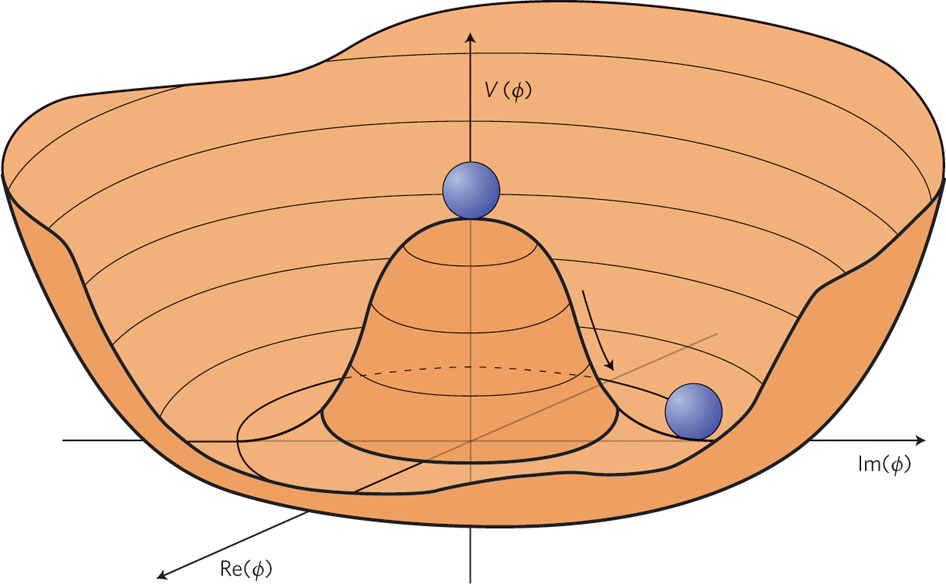
\includegraphics[width=0.5\textwidth]{figures/susyintro/higgspot_nature.jpg}
	\caption{The shape of the Higgs potential, from \cite{Ellis:higgs}}
	\label{fig:higgspot}
\end{figure}
This potential has a circle of degenerate energy at the field value $|\phi| = (-\mu^2/2\lambda)^{1/2}$, or in terms of the actual complex field, $\phi = (-\mu^2/2\lambda)^{1/2}e^{i\theta}, \, \theta \in [0,2\pi)$. The mechanism of {\it spontaneous symmetry breaking} occurs when, as the energy decreases, the Higgs field falls to the bottom of the degenerate circle and is forced to {\it choose} a particular value of $\theta$. This breaks the gauge invariance of the Lagrangian under both $U(1)_Y$ and $SU(2)_L$, and causes the gauge bosons of the two groups to mix together: The $B^\mu$ field mixes with $W^\mu_3$ to form the fields $A^\mu$ and $Z^\mu$, by the assignments
\begin{align}
	W_3^\mu &= \cos\theta_W Z^\mu + \sin\theta_W A^\mu,\\
	B^\mu &= -\sin\theta_W Z^\mu + \cos\theta_W A^\mu,
\end{align}
where $\theta_W$ is the {\it Weinberg angle}. The two other $SU(2)_L$ gauge fields, $W_{1,2}^\mu$, mix togeher to form
\begin{align}
	W_\mu = \frac{1}{\sqrt{2}} \left[ W_1^\mu - iW_2^\mu \right]
\end{align}
and its adjoint $(W^\mu)^\dag$. The field $A^\mu$ is the photon field, $Z^\mu$ is the Z boson field and $W^\mu/(W^{\mu\dag})$ is the $W^\pm$ bosons. The mixing restores the symmetry under a different $U(1)$ group, $U(1)_\mathrm{em}$, and the corresponding conserved charge is the electrical charge. The photon and Z boson are electrically netural, while the $W^\pm$ carry plus/minus one elementary unit of charge.\marginpar{Say something about vacuum expectation values}

The Higgs mechanism also provides fermionic terms of the form $\psi_i y_{ij} \psi_j$. For $i=j$, these are mass terms of the form written in the Dirac bilinear, eq. \eqref{eq:diracbilinear}, and for $i\neq j$ they give rise to off-diagonal terms in the CKM and PMNS matrices. The coupling constants of these terms are called {\it Yukawa couplings}.

\subsection{The Feynman calculus and loop corrections}
\label{subsec:feynmancalculus}
Very few problems in the framework of the Standard Model can be solved exactly. Instead, calculations are done using perturbation theory to series expand the solution as a sum of increasingly complicated, but decreasingly important, contributions. Feynman invented a technique for visualizing these expansions using visual diagrams, known as Feynman diagrams. For instance, the problem of inelastic electron-positron scattering has as its leading contribution the diagram shown in fig. \ref{fig:feynmandiagram_a}. The next-to-leading order includes the diagrams in figs. \ref{fig:feynmandiagram} (b), (c) and (d).
\begin{figure}[htbp]
	\centering
	\begin{subfigure}[b]{0.45\textwidth}
		\centering
		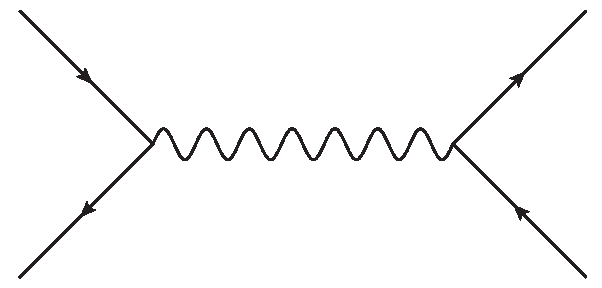
\includegraphics[width=0.6\textwidth]{figures/susyintro/epscattering.pdf}
		\caption{ }
		\label{fig:feynmandiagram_a}
	\end{subfigure}
	\begin{subfigure}[b]{0.45\textwidth}
		\centering
		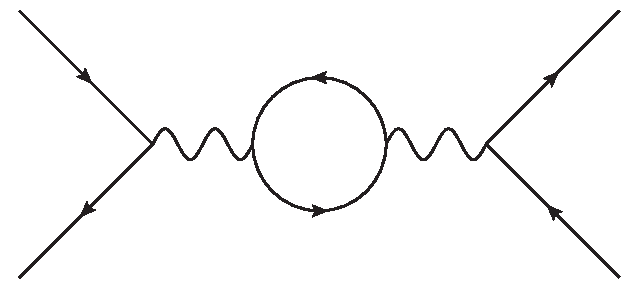
\includegraphics[width=0.6\textwidth]{figures/susyintro/epscattering_fermionloop.pdf}
		\caption{ }
		\label{fig:feynmandiagram_b}
	\end{subfigure}

	\begin{subfigure}[b]{0.45\textwidth}
		\centering
		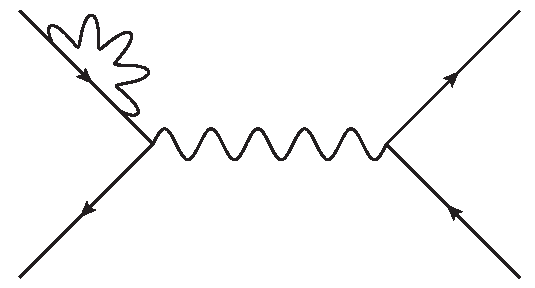
\includegraphics[width=0.6\textwidth]{figures/susyintro/epscattering_fermioncorr.pdf}
		\caption{ }
		\label{fig:feynmandiagram_c}
	\end{subfigure}
	\begin{subfigure}[b]{0.45\textwidth}
		\centering
		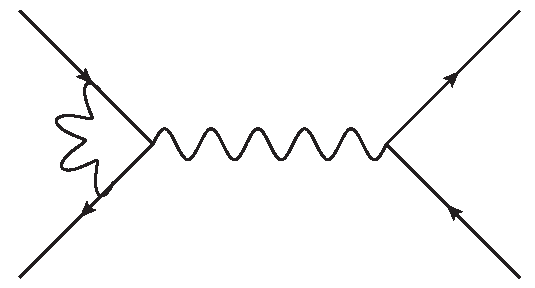
\includegraphics[width=0.6\textwidth]{figures/susyintro/epscattering_vertexcorr.pdf}
		\caption{ }
		\label{fig:feynmandiagram_d}
	\end{subfigure}
	\caption{Feynman diagrams of contributions to inelastic $e^+ e^-$ scattering. Made using \cite{Binosi:2003yf}.}
	\label{fig:feynmandiagram}
\end{figure}
The Feynman calculus associates each diagram with a specific mathematical expression called the Feynman amplitude $\mathcal{M}$ for that diagram. When several diagrams are included, the total amplitude for the process is the sum of the amplitudes from each diagram. The physical quantities of interest are obtained by integrating the amplitude (or its absolute square) over all spin and momentum configurations of the system.

\subsection{Renormalization}
The subleading diagrams, like those in fig.  \ref{fig:feynmandiagram} (b--d), contain closed loops. These loops introduce extra momentum integrals into the calculations. Often, these integrals are divergent -- which is unacceptable from a physical viewpoint. The divergences can be understood and dealt with by using the techniques of {\it regularization} and {\it renormalization}. 
\subsubsection{Regularization}
Regularization is a means for parametrizing the divergence in terms of some small parameter $\epsilon$ which is zero in the physical limit. The most modern way to regularize a momentum integral is by using {\it dimensional regularization}: The original loop integral is an integral over four space-time dimensions. Dimensional regularization makes the substitution $4 \to d = 4-\epsilon$, so the integral becomes
\begin{align}
	\int d^4 \, k \to \int d^d \, k.
\end{align}
This integral is mathematically well-defined, and allows the divergences to be parametrized in terms of $\epsilon$.
\subsubsection{Renormalization}
When the divergence has been isolated and parametrized, it needs to be explained physically. This is done by the process of renormalizing the theory. For instance, in the case of the photon propagator in quantum electrodynamics, illustrated in fig. \ref{fig:feynmandiagram_b}, the regularized expression for the leading-order loop correction to the propagator is proportional to
\begin{align}
	\frac{2}{\epsilon} + \mathrm{finite terms}, \label{eq:divergent_loop_result}
\end{align}
which blows up as $\epsilon\to 0$. Renormalization is the claim that this infinity is a part of the {\it bare} physical constants which are present in the Lagrangian, in this case the electrical charge, whose bare value is denoted $e_0$. These bare parameters are not observable quantities, only parameters in the Lagrangian. What is observed is the {\it renormalized} charge $e = e_0 + \delta e$, where $\delta e$ is the infinite shift contributed from eq. \eqref{eq:divergent_loop_result}.

All the coupling constants of the Standard Model get renormalized. The renormalization introduces an {\it energy dependence} into the coupling constants, since the shift comes from loop corrections which depend on the energy of the process. For instance, the physical value of the electron charge in quantum electrodynamics, at some momentum $q$, is given as
\begin{align}
	e^2(q) = \frac{e_r^2}{1 - (e_r^2/6\pi^2)\log(q/M)},\label{eq:electron_charge_running}
\end{align}
where $e_r$ is some referance value for the charge, defined at the energy scale $M$. The fact that the coupling constants are not constant is referred to as the {\it running of the coupling constants}.

\subsubsection{The Callan-Symanzik equation}
The Callan-Symanzik, or {\it renormalization group} equation is the equation which describes the running of the coupling constants in a systematic way for any interaction in a quantum field theory. It is obtained by requiring that the Greens function for the interaction, $G$, {\it i.e.}\ the propagator, varies with the renormalization scale $M$ in such a way that the bare parameters of the Lagrangian is unchanged. For the example of QED, the Callan-Symanzik equation for a Green's function with $n$ electron fields and $m$ photon fields is
\begin{align}
	\left[ M \frac{\partial}{\partial M} + \beta(e) \frac{\partial}{\partial e} + n\gamma_2(e) + m\gamma_3(e)\right] G^{(n,m)}(\{ x_i\}; M,e) = 0.\label{eq:callansymanzik}
\end{align}
The functions $\beta$ and $\gamma$ are defined as
\begin{align}
	\beta \equiv \frac{M}{\delta M} \delta e, \, \gamma_i \equiv - \frac{M}{\delta M}\delta \eta_i,
\end{align}
where $\delta\eta_i$ is the field-strength renormalization term, shifting the field values of the electron and photon fields,
\begin{align}
	\psi \to (1 + \delta \eta_2) \psi \, \mathrm{and} \, A_\mu \to (1 + \delta\eta_3) A_\mu,
\end{align}
respectively. The Callan-Symanzik equation states that the combined effect of all the shifts in parameters induced by the renormalization should exactly weigh up for the shift in the Green's function itself, which is given by
\begin{align}
	G^{(n,m)} \to (1 + n\delta\eta_2 + m\delta\eta_3)G^{(n,m)}.
\end{align}
This is what is stated in eq.\ \eqref{eq:callansymanzik}. The Callan-Symanzik equation for other interactions, such as the $SU(3)$ quantum chromodynamics, may be derived similarily, but its complexity grows with the complexity of the interaction.

The primary quantities of interest from a phenomenological viewpoint are the $\beta$ and $\gamma$ functions. They describe the change in the coupling constant and other parameters as a function of renormalization scale, and in the case of QED they may be used to derive the formula \eqref{eq:electron_charge_running} for the running of the electromagnetic coupling constant $e$. Equation \eqref{eq:electron_charge_running} shows that the electromagnetic coupling constant increases as a function of the energy $q$. The same turns out to be true for the weak coupling constant, while the strong coupling constant of QCD decreases with increasing energy. This last fact is called {\it asymptotic freedom}, and means that the quarks and gluons are unbound by strong forces in the limit of high energy. 





\section{Motivations for extending the Standard Model}

Since the Standard Model is widely believed to be a low-energy effective model of some more fundamental high-energy regime, it is speculated that the three interactions of the Standard Model unite at a higher energy and act as a single interaction under some larger gauge group. However, when the three couplings are evolved to high energies using the Callan-Symanzik equations, they do not meet at a single point. This is seen by many as a flaw of the Standard Model. In the theory of Supersymmetry, the evolution of the couplings is altered, and they do meet at a single point. This is shown in fig. \ref{fig:coupling_unification}. Supersymmetry is discussed in detail in the next chapter.
\begin{figure}[hbt]
	\centering
	\includegraphics[width=0.6\textwidth]{figures/susyintro/unification.eps}
	\caption{Evolution of the inverse coupling constants, for the cases of the Standard Model (dashed lines) and models with supersymmetry (solid lines). From \cite{Martin:1997ns}.}
	\label{fig:coupling_unification}
\end{figure}

Another issue with the Standard Model is that is has no candidate for particle dark matter. Observations over the last century have given strong evidence for the existence of some as yet unkown form of matter which is distributed in large quantites all over the universe -- in fact four times as much as our ordinary matter. It is widely believed that this dark matter is some form of particle. Dark matter interacts primarily, or possibly even solely, via gravitation, so the particle has to be colourless and electrically neutral, because the strength of these interactions would otherwise lead to the particle having been observed by now. It also has to be long-lived in order to explain the abundance of dark matter that we observe in the universe today, because the assumption is that it was thermally produced in the early universe and subsequently cooled off. These restrictions rule out most of the Standard Model particles, with the exception of neutrinos. But neutrinos are known to be very light, almost massless, and calculations of early-universe dynamics show that they are too light to be candidates for dark matter. 

There is also a more technical problem with the Standard Model, related to the scalar Higgs field. As discussed in section \ref{subsec:feynmancalculus}, the calculations of parameters in a quantum field theory are subject to loop corrections. The Higgs mass parameter recieves corrections from loops containing all massive particles, with the largest contribution coming from the top quark. These contributions are many orders of magnitude larger than the observed Higgs mass of 126 GeV, meaning that there must be cancellations among the correction terms. There is no symmetry in the Standard Model which says that such a cancellation should occur, so it appears to be an ``accident'' of nature. Such accidents are seen as very unnatural, and this explanation is thus very unsatisfactory from a theoretical viewpoint. This is called the {\it hierarchy problem}. In supersymmetry, the new degrees of freedom enter into the loop corrections, and because of the symmetry, they cancel the Standard Model contributions in a natural way. 



% The Standard Model is a quantum field theoretic model and may be stated in terms of a Lagrangian density function $\mathcal{L}$. The features that define the Standard Model emerge by requiring that it is invariant under the action of certain {\it gauge groups} -- specifically the infamous $U(1)_Y\times SU(2)_L\times SU(3)_C$, where the subscripts stand for {\it hypercharge, left} and {\it colour}, respectively, and refer to the properties that the different fields must have in order to be acted upon by the group transformations. By inserting certain {\it fermionic} field content in the Lagrangian and imposing these symmetries, the model acquires a number of {\it gauge bosons} for the different gauge groups. All these particles are {\it a priori} massless, a requirement to fulfill the gauge symmetry. To give particles their observed mass, then, one adds a scalar field and a corresponding scalar potential of a certain shape. The shape of the potential is such that the $U(1)_Y\times SU(2)_L$ symmetry is {\it spontaneously broken} at a certain energy scale, shifting the degrees of freedom around to give a scalar Higgs boson along with the other gauge bosons, and also giving mass to all particles except the photon. The remaining unbroken symmetries are then the $U(1)_\mathrm{em}$ for electromagnetic and $SU(3)_C$ for strong interactions. 



% The particles that make up the Standard Model are: the three generations of charged leptons, electron, muon and tau, and their three neutral counterparts, the neutrinos; the three generations of up- and down-type quarks up, down, charm, strange, top and bottom; the electroweak gauge bosons photon, Z and W; the strong gauge bosons, the gluons; and the Higgs boson. 





%%%%%%%%%%%%%%%%%%%%%%%%%%%%%%%%%%%%%%%%%%%%%%%%%%%%%%%%%%%%%%%%%%%%%%%%
\chapter{Supersymmetry}%%%%%%%%%%%%%%%%%
%%%%%%%%%%%%%%%%%%%%%%%%%%%%%%%%%%%%%%%%%%%%%%%%%%%%%%%%%%%%%%%%%%%%%%%%
\label{ch:susyintro}
The theory of supersymmetry (SUSY) is a proposed extension of the Standard Model which increases the number of degrees of freedom by introducing a symmetry between fermions and bosons, called a supersymmetry. The construction of supersymmetry is in some sense a two-step process, where one first derives the Lagrangian of a theory with complete symmetry between fermions and bosons, meaning that every bosonic degree of freedom gets a corresponding `supersymmetric' fermionic degree of freedom, and {\it vice versa}. These fields only differ in spin. But since {\it e.g.}\ scalar, colour charged particles with the same mass as the quarks are not observed in experiments, the symmetry cannot be exact. To make the theory physically viable, the supersymmetric partners must be significantly heavier than their Standard Model counterparts. This means that the supersymmetry must be a broken symmetry, and this breaking is put into the theory ``by hand''.

In this chapter we will outline the construction of a supersymmetric theory. First, we introduce the group theoretic framework of the symmetries. We define the concept of superfields, fields transforming under representations of the supersymmetry group. We go on to construct a fully supersymmetric Lagrangian in the framework of the Minimal Supersymmetric Standard Model (MSSM). Then the breaking of SUSY is achieved by manually inserting so-called ``soft'' SUSY-breaking terms. Also, the concept of R-parity is introduced in order to ensure the stability of the proton. R-parity will also make the lightest supersymmetric particle a good dark matter candidate. From the broken SUSY Lagrangian, we extract the particle content -- identifying the familiar fields of the Standard Model as well as their supersymmetric counterparts. We then introduce popular phenomenological models used to constrain and study the parameter space of the MSSM, and discuss their implications for the hierarchy of SUSY masses. This type of constrained model is subsequently adapted for the study of particular chain decays, which is the topic for the remainder of the thesis. We will also review the current experimental status of SUSY. 

The presentation is based on \cite{Batzing:2013} and \cite{Leinonen:2014}.

\section{Extending the Poincar\'{e} symmetry}
In the beginning of Chapter \ref{ch:SM_intro}, the Poincar\'{e} group was discussed. It is the group of all Lorentz boosts and rotations, as well as all translations in spacetime. Any physical theory obeying Special Relativity must be invariant under the Poincar\'{e} group. It was shown in 1967 by Coleman and Mandula \cite{PhysRev.159.1251} that there exists no extension of the Poincar\'{e} symmetry which includes the gauge groups of the Standard Model in a non-trivial way, {\it i.e.}\ a way by which the extended group cannot be decoupled as a direct product such that the groups do not couple to each other. 

This prompted Haag, \L{}opusza\'{n}ski and Sohnius \cite{Haag1975257} to introduce the concept of a {\it superalgebra}. A superalgebra is a direct product of two Lie algebras with a binary operation that mixes the algebras together. Haag {\it et.al.}\ constructed a superalgebra by combining the Lie algebra of the Poincar\'{e} group with an algebra spanned by four operators called {\it Majorana spinor charges}, represented by a two-component Weyl spinor $Q_A$ (to be defined shortly) and its hermitian conjugate $\bar Q_{\dot A}$. The resulting superalgebra is given by the (anti)commutation relations
\begin{align}
	[Q_A,P_\mu] =& [\bar Q_{\dot A}] = 0,\\
	[Q_A, M_{\mu\nu}] =& \sigma_{\mu\nu,A}^B Q_B,\\
	\{Q_A, Q_B\} =& \{\bar Q_{\dot A}, \bar Q_{\dot B} \} = 0,\\
	\{Q_A, \bar Q_{\dot B} \} =& 2\sigma^\mu_{A \dot B} P_\mu,\\
\end{align}
where $P_\mu$ is the momentum operator (the generator of translations in the Poincar\'{e} group), $M_{\mu\nu}$ are the generators of Lorentz boosts and rotations, $\sigma_\mu = (1,\sigma_i)$ with $\sigma_i$ the Pauli matrices and $\sigma_{\mu\nu} = \frac{i}{4}(\sigma_\mu \bar\sigma_\nu - \sigma_\nu \bar\sigma_\mu)$. 

In the usual representation of the Poincar\'{e} group, the fermion fields are represented as four-component Dirac spinors. It can be shown that the Poincar\'{e} group is isomorphic to $SL(2,\mathbb{C})$, so it is possible to work with representations of this group instead. The $SL(2,\mathbb{C})$ group has two inequivalent fundamental representations by two-component spinors which are called {\it left- and right-handed Weyl spinors} and written as $\psi_A$ and $\bar\psi_{\dot A}$, respectively. 

The transformations corresponding to the superalgebra are called {\it supersymmetry transformations}.

\section{Superfields}
The representations of the objects transforming under the supersymmetry transformations are called superfields. There are two important types, called chiral/scalar and vector superfields. The superfields are expressed in terms of spacetime coordinates $x^\mu$ and four anti-commuting Grassman numbers $\theta_A$ and $\bar\theta_{\dot A}$. Together, these eight coordinates form the {\it superspace}. Because of the anticommutativity, which means that any Grassman number squared vanishes, a function of a Grassman number, $f(\theta_A)$, has an all-order expansion given by
\begin{align}
	f(\theta) = a + b\theta_A.
\end{align}
Using this fact, a superfield $\Phi$ may generally be written as
\begin{align}
	\Phi = &f(x) + \theta^A\phi_A(x) + \bar\theta_{\dot A}\bar\chi^{\dot A}(x) + \theta \theta m(x)\\
	 &+ \bar\theta \bar\theta n(x) + \theta\sigma^\mu \bar\theta V_\mu(x) + \theta\theta\bar\theta_{\dot A}\bar\lambda^{\dot A}(x) + \bar\theta \bar\theta \theta^A \psi_A(x) + \theta \theta \bar\theta \bar\theta d(x).\nonumber
\end{align}
The different field components have the following properties: $f(x)$, $m(x)$ and $n(x)$ are complex (pseudo)scalars, $\psi_A(x)$ and $\phi_A(x)$ are left-handed Weyl spinors, $\bar\chi^{\dot A}(x)$ and $\bar\lambda^{\dot A}(x)$ are right-handed Weyl spinors, $V_\mu (x)$ is a Lorentz four-vector and $d(x)$ is a complex scalar.
% \begin{itemize}
% 	\item $f(x), m(x)$ and $n(x)$ are complex (pseudo)scalars
% 	\item $\psi_A(x)$ and $\phi_A(x)$ are left-handed Weyl spinors
% 	\item $\bar\chi^{\dot A}(x)$ and $\bar\lambda^{\dot A}(x)$ are right-handed Weyl spinors
% 	\item $V_\mu (x)$ is a Lorentz four-vector
% 	\item $d(x)$ is a complex scalar
% \end{itemize}

 A set of covariant derivatives are defined by
\begin{align}
	D_A = \frac{\partial}{\partial \theta^A} - i\sigma^\mu_{A \dot A}\bar\theta^{\dot A}\partial_\mu, \, \bar D^{\dot A} = -\frac{\partial}{\partial \bar \theta_{\dot A}} + i\bar\sigma^{\mu,A \dot A}\theta_A \partial_\mu.
\end{align}
In terms of these, a {\it left chiral} superfield $\Phi$ is defined by the condition.
\begin{align}
	\bar D^{\dot A} \Phi = 0.
\end{align}
By substituting $y^\mu = x^\mu - i\theta\sigma^\mu \bar \theta$, the covariant derivative $\bar D^{\dot A}$ is given as
\begin{align}
	\bar D^{\dot A} = -\frac{\partial}{\partial \bar\theta_{\dot A}}.
\end{align}
This shows that a left-chiral superfield must be independent of $\bar \theta$ in these coordinates, so it may generally be written as
\begin{align}
	\Phi(y, \theta) = A(y) + \sqrt{2}\theta\psi(y) + \theta\theta F(y), 
\end{align}
thus containing two complex scalar fields and a left-handed Weyl spinor. Under an infinitesimal supersymmetry transformation
\begin{align}
	\delta_\xi \Phi = -i(\xi Q + \bar\xi\bar Q)\Phi,
\end{align}
the component field $F$ can be shown to transform into a total derivative. It will thus not contribute to the action, since all fields must vanish on the boundary at infinity. For this reason it is called an auxillary field. Thus we see that a left-chiral superfield contains two bosonic (scalar) degrees of freedom and two fermionic degrees of freedom contained in a left-handed Weyl spinor. Similar arguments may be applied to define a right-chiral superfield by the condition
\begin{align}
	D_A \Psi^\dag = 0,
\end{align}
and to show that it contains two auxillary and two proper scalar degrees of freedom, as well as a right-handed Weyl spinor. 

A {\it vector superfield} is defined by the condition
\begin{align}
	\Phi^\dag = \Phi.
\end{align}
This condition allows the field content, for a general vector superfield $V$,
\begin{align}
	V = &f(x) + \theta^A\phi_A(x) + \bar\theta_{\dot A}\bar\chi^{\dot A}(x) + \theta \theta m(x) + \bar\theta \bar\theta m^*(x)\\
	 &+ \theta\sigma^\mu \bar\theta V_\mu(x) + \theta\theta\bar\theta_{\dot A}\bar\lambda^{\dot A}(x) + \bar\theta \bar\theta \theta^A \lambda_A(x) + \theta \theta \bar\theta \bar\theta d(x).
\end{align}
Here, the scalar fields $f(x)$ and $d(x)$, as well as the four-vector $V_\mu (x)$, are required to be real fields, thus halving their amount of degrees of freedom. There are auxillary degrees of freedom which may be removed by a gauge transformation. A vector superfield may be written in the {\it Wess-Zumino} gauge as
\begin{align}
	V_\mathrm{WZ} = (\theta \sigma^\mu \bar\theta) \left[ V_\mu(x) + i\partial_\mu (A(x) - A^*(x)) \right] + \theta\theta \bar\theta_{\dot A} \bar\lambda^{\dot A}(x) + \bar\theta \bar\theta \theta_A \lambda^A(x) + \theta\theta \bar\theta \bar\theta d(x).
\end{align}
In this gauge, the vector superfield contains one real scalar field degree of freedom (d.o.f.), three gauge field d.o.f.'s and four fermion d.o.f.'s.

\section{The unbroken SUSY Lagrangian}
To obtain a theory which is supersymmetric, the action, given by
\begin{align}
 	S = \int d^4 x \mathcal{L},
 \end{align}
 needs to be invariant under SUSY transformations. As mentioned in the previous section, a total derivative has this property because it is determined by the boundary conditions, where it has to vanish. It can be shown that the highest-order component fields in $\theta$ and $\bar \theta$, {\it i.e.}\ the term proportional to $\theta\theta\bar\theta\bar\theta$, always has this property for both chiral and vector superfields and products thereof. Thus the invariance of the action may be ensured by redefining the Lagrangian such that
 \begin{align}
 	S = \int d^4 x \int d^4 \theta \mathcal{L},
 \end{align}
 where the last integral is over the four Grassman variables. This will project out only the desired terms, because of how the Grassman integral is defined. Thus the supersymmetric Lagrangian may be constructed from superfields and their products.

 A {\it superpotential} is defined as a product of left-chiral superfields,
 \begin{align}
 	W(\Phi) = L^i\Phi_i + \frac{1}{2}m^{ij}\Phi_i\Phi_j + \frac{1}{3}\lambda^{ijk}\Phi_i\Phi_j\Phi_k.
 \end{align}
The inclusion of higher-order field terms are forbidden from the condition of renormalizability, which forbids terms where the combined mass dimension of the fields are larger than four. Scalar, fermionic and auxillary fields have mass dimension one, 3/2 and 2, respectively. A fourth order superfield term would include field terms which break this condidtion. The most general Lagrangian that can be written in terms of chiral superfields is
\begin{align}
	\mathcal{L} = \Phi_i^\dag \Phi_i + \bar\theta\bar\theta W(\Phi) + \theta\theta W(\Phi^\dag),
\end{align}
where the first term is called the kinetic term. 

The Lagrangian has to be gauge invariant. The general gauge transformation of a chiral superfield under a group $G$ is given by
\begin{align}
	\Phi \overset{G}{\to} e^{-iq\Lambda^a T_a}\Phi
\end{align}
where $T_a$ are the group generators, $q$ is the charge of $\Phi$ under $G$ and the gauge parameters $\Lambda_a$ themselves can be shown to be left-chiral superfields. The equivalent transformation for a right-chiral superfield $\Phi^\dag$ involves a right-chiral superfield gauge parameter $\Lambda_a^\dag$.

Analogously to the Standard Model, the supersymmetric gauge interactions are introduced as compensating terms to the gauge transformation of the chiral superfields. The analogue to the gauge boson fields are the vector superfields $V^a$, which are introduced into the kinetic terms of the Lagrangian by writing them as
\begin{align}
	\Phi^\dag_i e^{q V^a T_a}\Phi_i,
\end{align}
such that the kinetic term transforms as
\begin{align}
	\Phi_i^\dag e^{q V^a T_a}\Phi_i \overset{G}{\to} \Phi^\dag e^{iq(\Lambda^a)^\dag T_a}e^{qV^{'a}T_a}e^{-iq\Lambda^a T_a}\Phi,
\end{align}
which is invariant given that the vector superfields transform as
\begin{align}
	e^{qV^{'a} T_a} = e^{-iq(\Lambda^a)^\dag T_a}e^{qV^a T_a}e^{iq\Lambda^a T_a}.
\end{align}
For infinitesimal $\Lambda$, this is to leading order
\begin{align}
	V^{'a} = V^a + i(\Lambda^a - (\Lambda^a)^\dag) - \frac{1}{2}qf^a_{bc} V^b ((\Lambda^c)^\dag + \Lambda^c).
\end{align}
This gives for the vector component fields of the vector superfields, $V_\mu^a$,
\begin{align}
	V^a_\mu \overset{G}{\to} V^{'a}_\mu = V_\mu^a + i\partial_\mu(\Lambda^a - (\Lambda^a)^\dag) - qf^a_{bc} V_\mu^b (\Lambda^c + (\Lambda^{c})^\dag).
\end{align}
With these definitions, it can be shown that the Standard Model couplings of fermions with bosons are recovered by defining the covariant derivative
\begin{align}
	D_\mu^i = \partial_\mu - \frac{i}{2} q_i V_\mu.
\end{align}

The SUSY Lagrangian terms containing the field strengths of the gauge fields are written as
\begin{align}
	\mathrm{Tr}[W^A W_A],
\end{align}
called the supersymmetric field strength, where $W_A$ and $\bar W_{\dot A}$ are left- and right-handed chiral superfields, respectively, given by
\begin{align}
	W_A &\equiv -\frac{1}{4}\bar D\bar D e^{-qV^aT_a} D_A e^{qV^a T_a},\\
	\bar W_{\dot A} &\equiv -\frac{1}{4} D D e^{-qV^aT_a} \bar D_{\dot A} e^{qV^a T_a}.
\end{align}
The general form of the SUSY Lagrangian is
\begin{align}
	\mathcal{L} \Phi^\dag e^{qV^a T_a}\Phi + \bar\theta\bar\theta W(\Phi) + \theta\theta W(\Phi^\dag) + \frac{1}{2T(R)}\bar\theta \mathrm{Tr}(W^A W_A),
\end{align}
where $T(R)$, the {\it Dynkin index} of the representation of the gauge group, is a normalization constant.



\subsection{SUSY breaking}
Supersymmetry has to be a broken theory, at least in the low-energy limit, since supersymmetric particles with Standard Model masses are not observed. The breaking can be inserted into the SUSY Lagrangian ``by hand'', by explicitly adding terms that break SUSY and allow for mass splitting. The rationale for these terms is that the SUSY Lagrangian is only an effective Lagrangian where some heavy field has been integrated out, and that the breaking of SUSY occurs through this field at a higher scale. There are several alternatives for the mechanisms of SUSY breaking, some of which are Planck-scale mediated SUSY breaking, gauge mediated SUSY breaking and anomaly mediated SUSY breaking. Whichever of the mechanisms is chosen, there are only a finite set of terms that may be added to the Lagrangian without breaking renormalizability. They are called {\it soft} SUSY breaking terms, required to have couplings of mass dimension one or higher, and may in the most general form be written
\begin{align}
	\mathcal{L}_\mathrm{soft} = &-\frac{1}{4T(R)}M\theta\theta\bar\theta\bar\theta \mathrm{Tr} [W^A W_A] - \frac{1}{6}a_{ijk} \theta\theta\bar\theta\bar\theta\Phi_i \Phi_j \Phi_k\nonumber\\
	&-\frac{1}{2}b_{ij} \theta\theta\bar\theta\bar\theta\Phi_i \Phi_j - t_i \theta\theta\bar\theta\bar\theta \Phi_i + \mathrm{h.c.}\\
	&-m_{ij} \theta\theta\bar\theta\bar\theta \Phi_i^\dag \Phi_j.\nonumber
\end{align}
In terms of the component fields of the superfields, the soft Lagrangian may be written
\begin{align}
	\mathcal{L}_\mathrm{soft} = &-\frac{1}{2} M\lambda^A\lambda_A - \left( \frac{1}{6} a_{ijk} A_i A_j A_k + \frac{1}{2} b_{ij} A_i A_j + t_i A_i + \frac{1}{2} c_{ijk} A^*_i A_j A_k + \mathrm{c.c.}\right)\\
	&- m_{ij}^2 A_i^* A_j.\nonumber
\end{align}
Since this contains both Weyl spinor fields and scalar fields, the soft terms may be used to modify masses and couplings of the superpartner scalar and fermionic fields which will appear in a moment.



\section{The Minimal Supersymmetric Standard Model}
The Minimal Supersymmetric Standard Model (MSSM) is the minimal supersymmetric theory which contains the Standard Model. It is constructed by choosing field content in accordance with the requirements deduced in the previous sections. To construct a Dirac fermion, we use one left-chiral and one right-chiral superfield together. This gives the four fermionic degrees of freedom that a Dirac fermion and its antiparticle require. Since each chiral superfield also contains two scalar degrees of freedom (after removing the auxillary fields), this introduces two scalar particle-antiparticle pairs, which are called the supersymmetric partners, or {\it superpartners}, of the Dirac fermion. An important point is that all superfield components must have the same charge under all gauge groups, due to the way the gauge transformation was defined. This means that the scalar fields generally will be charged. For instance, the superfields for the charged leptons are denoted $l_i$ and $\bar E_i$ for the left- and right-chiral superfields, respectively, and the left-handed neutrino superfields are denoted $\nu_i$. Here, $i=1,2,3$ is a generation index. The $SU(2)_L$ doublet of the Standard Model is recovered by setting $L_i = (\nu_i, l_i)$. The quark superfields are denoted $u_i$, $\bar U_i$, $d_i$ and $\bar D_i$, where $Q_i = (u_i, d_i)$ makes the $SU(2)_L$ doublet.

The gauge boson fields come from the vector superfields, each of which also contains two Weyl-spinor fields of opposite handedness. To obey gauge invariance, $n^2-1$ vector superfields are required for each of the $SU(n)$ groups just as in the Standard Model -- {\it i.e.}\ gauge invariance under $U(1)_Y\times SU(2)_L \times SU(3)_C$ requires 1+3+8 vector superfields.\footnote{Again, $n^2$ rather than $n^2-1$ for the $U(1)$ group.} These are denoted $B^0$, $W^a$ and $C^a$, respectively. The Weyl spinor fields, corresponding to superpartners of the gauge fields, are written as $\tilde B^0$, $\tilde W^0$ and $\tilde g$, respectively. In the literature, these are referred to as {\it bino}, {\it wino} and {\it gluino}. 

The MSSM requires two Higgs superfield $SU(2)_L$ doublets to be able to give mass to both up- and down-type quarks. In the Standard Model, the same Higgs doublet can be used for both types by rotating the components using the $SU(2)_L$ generators, but this is not possible in SUSY. The Higgs doublets in the MSSM are
\begin{align}
	H_u = \begin{pmatrix}
		H_u^+ \\ H_u^0
	\end{pmatrix}, \, H_d = \begin{pmatrix}
		H_d^0 \\ H_d^-
	\end{pmatrix}.
\end{align}
This introduces several additional Higgs scalars into the model, as well as the fermionic superpartner fields.

The fields listed above come together and construct the MSSM Lagrangian $\mathcal{L}_\mathrm{MSSM}$ using the rules described above for a general gauge invariant SUSY Lagrangian, giving rise to kinetic terms, superpotential terms and supersymmetric field strength terms. The SUSY breaking soft terms of the MSSM are, in component fields,
\begin{align}
	&\left( -\frac{1}{2}M_1 \tilde B \tilde B - \frac{1}{2}M_2 \tilde W^{i,A} \tilde W^i_A - \frac{1}{2}M_3 \tilde g^{a,A}\tilde g^a_A + \mathrm{c.c.} \right)\nonumber\\
	+ &\left(-a_{ij}^e \tilde L_i H_d {\tilde e^*}_{iR} - a_{ij}^u \tilde Q_i H_u \tilde u^*_{iR} - a_{ij}^d \tilde Q_i H_d \tilde d^*_{jR} + \mathrm{c.c.} \right)\\
	- &(m_{ij}^L)^2 \tilde L_i^\dag \tilde L_j - (m_{ij}^e)^2 {\tilde e_{iR}^*} {\tilde e_{jR}} - (m_{ij}^Q)^2 \tilde Q_i^\dag \tilde Q_j \nonumber \\
	- &(m_{ij}^u)^2 {\tilde u_{iR}^*} {\tilde u_{jR}} - (m_{ij}^d)^2 {\tilde d_{iR}^*} {\tilde d_{jR}} - m^2_{H_u} H^\dag_u H_u - m^2_{H_d} H^\dag_d H_d.\nonumber
\end{align}
These terms constitute the main contributions to the superpartner masses.

The Lagrangian will {\it a priori} contain terms which break lepton and baryon number conservation, such as $LH_u$, $LLE$ and $LQ\bar D \in \mathcal{L}_\mathrm{MSSM}$. If the couplings for these terms are large, they allow for proton decay, which is experimentally very heavily constrained, with a lifetime of $\tau_\mathrm{proton} > 10^{33} \,\mathrm{yr}$. To avoid this, it is conventional to introduce the concept of {\it R-parity}, which gives an explanation for why these terms are zero.

\subsection{R-parity}
R-parity is a multiplicative quantum number which is assumed to be conserved in all SUSY interactions. Formally, a particle has R-parity given by
\begin{align}
	R = (-1)^{2s + 3B + L},
\end{align}
where $s$ is the particle's spin, $B$ its baryon number and $L$ its lepton number. The important point is that all Standard Model particles have $R=+1$ while all superpartners have $R = -1$. This leads to the very important prediction that superpartner particles only can be produced and annihilated in pairs. In particular, it means that the lightest superpartner (LSP) must be stable against decay. This makes the LSP very attractive as a candidate for dark matter, if it is electrically neutral.

\subsection{Radiative electroweak symmetry breaking}
Like any quantum field theory, the MSSM is subject to renormalization, which induces the running of the coupling constants and masses of the model as discussed in Chapter \ref{ch:SM_intro}. In particular, the mass parameters $m_{H_u/d}$ for the Higgs doublets, which come from soft breaking terms in the Lagrangian, run with energy. To break the electroweak symmetry, it is assumed that these are equal at some high scale, and run down. It can be shown that the running is proportional to the Yukawa couplings of the third-generation quarks of the respective type -- {\it i.e.}\ the top and bottom, respectively. Because the top Yukawa coupling is much larger than the bottom one, the $m_{H_u}$ parameter runs down much faster with energy and becomes negative. One can further show that this is a sufficient condition to induce the electroweak symmetry breaking, and thus give the gauge bosons and fermions their observed mass.\marginpar{Is this too ``dodgy''? Should I be more technical? I fear there are too many technicalities already.} 

In the course of the symmetry breaking, the neutral components of both the Higgs doublets acquire a non-vanishing vacuum expectation value, $v_u = \langle H_u^0 \rangle$ and $v_d = \langle H_d^0 \rangle$, respectively. These must relate to the vector boson masses of the Standard Model as
\begin{align}
	v_u^2 + v_d^2 = \frac{2m_Z^2}{g^2 + g^{'2}} \approx (174 \,\mathrm{GeV})^2.
\end{align}
The remaining free parameter is conventionally parametrized as
\begin{align}
	tan \beta \equiv \frac{v_u}{v_b}.
\end{align}

\subsection{Particle phenomenology of the MSSM}
The total particle content of the MSSM is as follows: 
\begin{itemize}
	\item The Standard Model particles are present: electrons, muons, taus and their corresponding neutrinos; the up, down, strange, charm, bottom and top quarks; the photon, Z boson and W bosons and gluons; and the Higgs boson.
	\item In addition to the Standard Model Higgs $h$, there are four other scalar Higgs particles with positive R-parity, labeled $H$, $H^\pm$ and $A$. $H$ is identical to $h$ except for its larger mass, and is therefore termed ``heavy Higgs'', in contrast to the ``light Higgs'' $h$ of the Standard Model. The other neutral field $A$ is a pseudo-scalar.
	\item All the Standard Model particles get superpartners, often termed {\it sparticles}:
	\begin{itemize}
	 	\item For the gluons, they are called gluinos and labeled $\tilde g$. 
	 	\item The partners of the $B^0$ and $W^a$ fields, which in the Standard Model form the photon, $Z$ and $W^\pm$, mix with the superpartner Higgs fields to form four neutral Majorana fermions called neutralinos, labeled $\tilde\chi_i^0$, $i=1,...,4$, and two charged fermion-antifermion pairs called charginos, $\tilde\chi_i^\pm$, $i=1,2$. 
	 	\item Each of the Standard Model fermions get two corresponding scalar particles with the same gauge charges. For the first two generations, the mass eigenstates split to good approximation into one left-chiral and one right-chiral fermion, such that {\it e.g.}\ the superpartners of the up quark $u$ are labeled $\tilde u_R$ and $\tilde u_L$. For the third-generation fermions, the chiral approximation is cruder, so these mass eigenstates are just numbered, {\it e.g.}\ $\tilde b_1$ and $\tilde b_2$ for the $b$ quark. 
	 \end{itemize} 
 \end{itemize}

 The superpartner fields are members of the same superfields as their standard model partners. Therefore, they inherit the couplings of their partners. This is very useful when drawing Feynman diagrams for processes, since intuition from the Standard Model can be applied through {\it supersymmetrization} of the diagrams. For instance, the {\it fermion-fermion-gauge boson} vertices (fig. \ref{fig:feynmandiagram_supersymmetrization_a}) of the Standard Model have supersymmetrized {\it fermion-sfermion-gaugino} versions (fig. \ref{fig:feynmandiagram_supersymmetrization_b}). (But not {\it sfermion-sfermion-gaugino}, because of R-parity.) 
 \begin{figure}[htbp]
	\centering
	\begin{subfigure}[b]{0.45\textwidth}
		\centering
		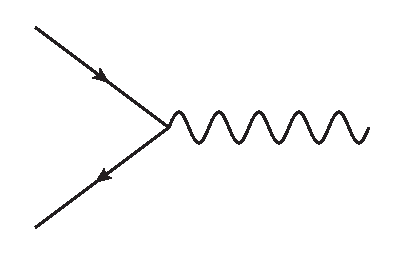
\includegraphics[width=0.6\textwidth]{figures/susyintro/ffg_vertex.eps}
		\caption{ }
		\label{fig:feynmandiagram_supersymmetrization_a}
	\end{subfigure}
	\begin{subfigure}[b]{0.45\textwidth}
		\centering
		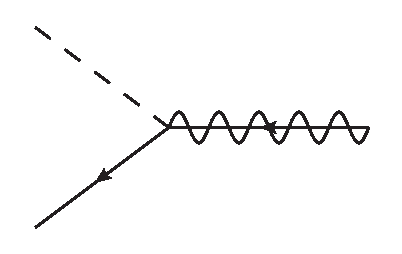
\includegraphics[width=0.6\textwidth]{figures/susyintro/sfg_vertex.eps}
		\caption{ }
		\label{fig:feynmandiagram_supersymmetrization_b}
	\end{subfigure}
	\caption{Feynman diagrams of a {\it fermion-fermion-gauge boson} vertex {\bf (a)} and the supersymmetrized {\it fermion-sfermion-gaugino} vertex {\bf (b)}.}
	\label{fig:feynmandiagram_supersymmetrization}
\end{figure}
An important consequence of the coupling inheritance is that the gaugino fields $\tilde\chi_i^{0/\pm}$ will couple differently depending on the mass mixing matrix. Since the wino field inherits the left-chiral $SU(2)_L$ coupling, the chirality of the couplings of the four neutralinos may differ considerably if the mass eigenstates are close to the gauge eigenstates. In the parameter point used for the analysis in the coming chapters, the second-generation neutralino consists of a large wino part, and this means that it couples weakly to right-chiral quarks. 

 \subsubsection{Sparticle masses}
 The main contributions to the sparticle masses naturally come from the soft terms, since these are responsible for the symmetry breaking which would otherwise give Standard Model masses to sparticles. The mass parameters from these terms are the gaugino mass terms $M_{1,2,3}$, the sfermion mass terms $m_{ij}$ and the Higgs terms $m_{H_{u/d}}$. Additionally, the parameter $\mu$ from the superpotential term coupling the Higgs doublets together in the unbroken SUSY Lagrangian contributes. Now follows a listing of some (s)particle masses, from \cite{Batzing:2013}.
 \begin{itemize}
 	\item At tree level, the different Higgs masses (which have positive R-parity) are
 	\begin{align}
 		m_A^2 &= 2|\mu|^2 + m^2_{H_u} + m^2_{H_d},\nonumber\\
 		m^2_{h,H} &= \frac{1}{2} \left( m_A^2 + m_Z^2 \pm \sqrt{(m_A^2 - m_Z^2)^2 + 4m_Z^2m_A^2\sin^2 2\beta} \right),\\
 		m^2_{H^\pm} &= m_A^2 + m_W^2.\nonumber
 	\end{align}
 	\item The gluino mass $m_{\tilde g}$ is given as
 	\begin{align}
 		m_{\tilde g} = M_3 \left[ 1 + \frac{\alpha_s}{4\pi}\left( 15 + 6\ln\frac{\mu}{M_3} + \sum_{\mathrm{all} \tilde q} A_{\tilde q} \right)\right],
 	\end{align}
 	where $A_{\tilde q}$ are the squark loop contributions given by
 	\begin{align}
 		A_{\tilde q} \int_0^1 dx \, x \ln\left( x \frac{m^2_{\tilde q}}{M_3^2} + (1-x)\frac{m_q^2}{M_e^2} - x(1-x) - i\epsilon \right).
 	\end{align}\marginpar{Not really sure what $M_e$ is...}
 	\item The neutralinos $\tilde\chi_i^0$ are the mass eigenstates of the bino, wino and higgsino fields. In the gauge eigenstate basis, where $\tilde\chi^{0T} = (\tilde B^0, \tilde W^0, \tilde H_d^0, \tilde H_u^0)$, the mass matrix may be written
 	\begin{align}
 		M_{\tilde \chi^0} = \begin{pmatrix}
 			M_1 & 0 & - c_\beta s_{\theta_W} m_Z &  s_\beta s_{\theta_W} m_Z \\
 			0 & M_2 &  c_\beta c_{\theta_W} m_Z & - s_\beta c_{\theta_W} m_Z\\
 			- c_\beta s_{\theta_W} m_Z &  s_\beta s_{\theta_W} m_Z & 0 & -\mu \\
			 c_\beta c_{\theta_W} m_Z & - s_\beta c_{\theta_W} m_Z & -\mu & 0
 		\end{pmatrix},
 	\end{align}
 	where $c_x = \cos x$ and $s_x = \sin x$. For a given parameter choice, this matrix must be diagonalized to find the neutralino masses.
 	\item The charginos $\tilde\chi_i^\pm$ have analogous structure. In the gauge eigenstate basis $\tilde \chi^{\pm T} = (\tilde W^+, \tilde H_u^+, \tilde W^-, \tilde H_d^-)$, the mass matrix is
 	\begin{align}
 		M_{\tilde \chi^\pm} = \begin{pmatrix}
 			0 & 0 & M_2 & \sqrt{2} c_\beta m_W  \\
 			0 & 0 & \sqrt{2} s_\beta m_W & \mu \\
 			M_2 & \sqrt{2} s_\beta m_W & 0 & 0\\
 			\sqrt{2} s_\beta m_W & \mu & 0 & 0
 		\end{pmatrix}.
 	\end{align}
 	\item The first two generations of {\it sfermions}, superpartners of the Standard Model fermions, get masses according to
 	\begin{align}
 		m^2_F = m^2_{F,\mathrm{soft}} + \Delta_F,
 	\end{align}
 	where $m^2_{F,\mathrm{soft}}$ is the mass term from the soft term of the form $-m^2_F F^\dag F$ and $\Delta_F$ is given by
 	\begin{align}
 		\Delta_F = (T_{3F} - Q_F \sin^2\theta_W)\cos 2\beta m^2_Z,
 	\end{align}
 	where $T_{3f}$, $Y$ and $Q$ are the weak isospin, hypercharge and electric charge, respectively, of the left-handed supermultiplet to which the sfermion belongs. The masses are then {\it e.g.}\
 	\begin{align}
 		&m^2_{\tilde e_L} = m^2_{L_1} + \Delta \tilde e_L,\\
 		&m^2_{\tilde e_R} = m^2_{e_R} + \Delta \tilde e_R.
 	\end{align}
 	The mass-splitting between same-generation sleptons and squarks are quark/lepton- and generation-independent and given by {\it e.g.}\ \marginpar{Is it the same for right-handeds? Check, or don't mention?}
 	\begin{align}
 		m^2_{\tilde e_L} - m^2_{\tilde \nu_L} = m^2_{\tilde d_L} - m^2_{\tilde u_L} = -\cos 2\beta m_W^2.
 	\end{align}
 	\item The third-generation sfermions get more complicated masses, given for {\it e.g.}\ the stop squark by the mass matrix (in the chiral gauge eigenstate basis $\tilde t^T = (\tilde t_L, \tilde t_R)$)
 	\begin{align}
 		m^2_{\tilde t} = \begin{pmatrix}
 			m^2_{Q_3} + m_t^2 + \Delta \tilde u_L & v(a_t^* \sin\beta - \mu y_t \cos\beta)\\
 			v(a_t \sin\beta - \mu^* y_t \cos\beta) & m^2_{u3} + m^2_t + \Delta \tilde u_R
 		\end{pmatrix},
 	\end{align}
 	which can be diagonalized to find the mass eigenstates.
 \end{itemize}

 \subsection{Gauge unification and mass hierarchies}
 It was mentioned in the introduction that one very appealing feature of supersymmetry is that the coupling constants of the electromagnetic, weak and strong interactions can be made to unite at a high energy scale. By assuming such a unification at the ``grand unification scale'' $m_\mathrm{GUT} \approx 2\times 10^{16} \,\mathrm{GeV}$, and evolving the SUSY parameters down to the low scale using the $\beta$ functions from the Callan-Symanzik equation, it can be shown that at a scale of 1 TeV, the ratio of the soft mass parameters $M_{1,2,3}$ is
 \begin{align}
 	M_3 : M_2 : M_1 = 6 : 2 : 1.
 \end{align}
 This propagates into the mass formulas to predict the approximate mass relationships
 \begin{align}
 	m_{\tilde g} \approx 6m_{\tilde \chi_1^0}, \, \mathrm{and} \, m_{\tilde \chi_2^0} \approx m_{\tilde \chi_1^\pm} \approx 2m_{\tilde \chi_1^0}.
 \end{align}

\section{The Constrained MSSM}
The available parameter space of the general MSSM is very large, of the order 100 free parameters. It is therefore conventional to make some restricting assumptions. A much-studied restriction is the {\it Constrained MSSM} (CMSSM), also known as {\it minimal supergravity} (mSUGRA). This model is constructed by assuming that SUSY breaking is mediated by some mechanism of gravity at the Planck scale of $M_P = 2.4\times 10^{18} \, \mathrm{GeV}$. By assuming a minimal form for the parameters at the GUT scale, to obtain gauge unification, the resulting model is parametrized in terms of five parameters,
\begin{align}
	m_{1/2}, \, m_{0}, \, A_0, \, \tan\beta \, \mathrm{and} \, \mathrm{sign}(\mu).
\end{align}
The mass parameters $m_{1/2}$ and $m_0$ are the common masses of all gauginos and sfermions, respectively, at the GUT scale. The mass splitting between sparticles appears when the individual sparticle masses are evolved down to a lower scale.
\begin{figure}[hbt]
	\centering
	\includegraphics[width=0.8\textwidth]{figures/susyintro/MSSMrun.eps}
	\caption{MSSM RGE running, from \cite{Martin:1997ns}.}
	\label{fig:mssm_rgerun}
\end{figure}
This is illustrated in fig. \ref{fig:mssm_rgerun} for one choice of $m_{1/2}$ and $m_0$. The figure also illustrates the evolution of $m_{H_u}$ down to a negative value, facilitating the radiative electroweak symmetry breaking.

Because the renormalization running, which is proportional to the mass of the Standard Model partners, the sfermion partners will often get an inverted mass hierarchy compared to the Standard Model. Especially in the colour sector, where stop and sbottom are often the lightest squarks. However, the effect may be compensated by other terms, and often the mass splittings are small.



\section{The experimental status of SUSY}
Include some ATLAS plots. Say something about $B_s \to \mu^+ \mu^-$ at LHCb and constraints on $\tan \beta$? Discuss mSUGRA validity. Mention more general naturalness condition?

\begin{figure}[hbt]
	\centering
	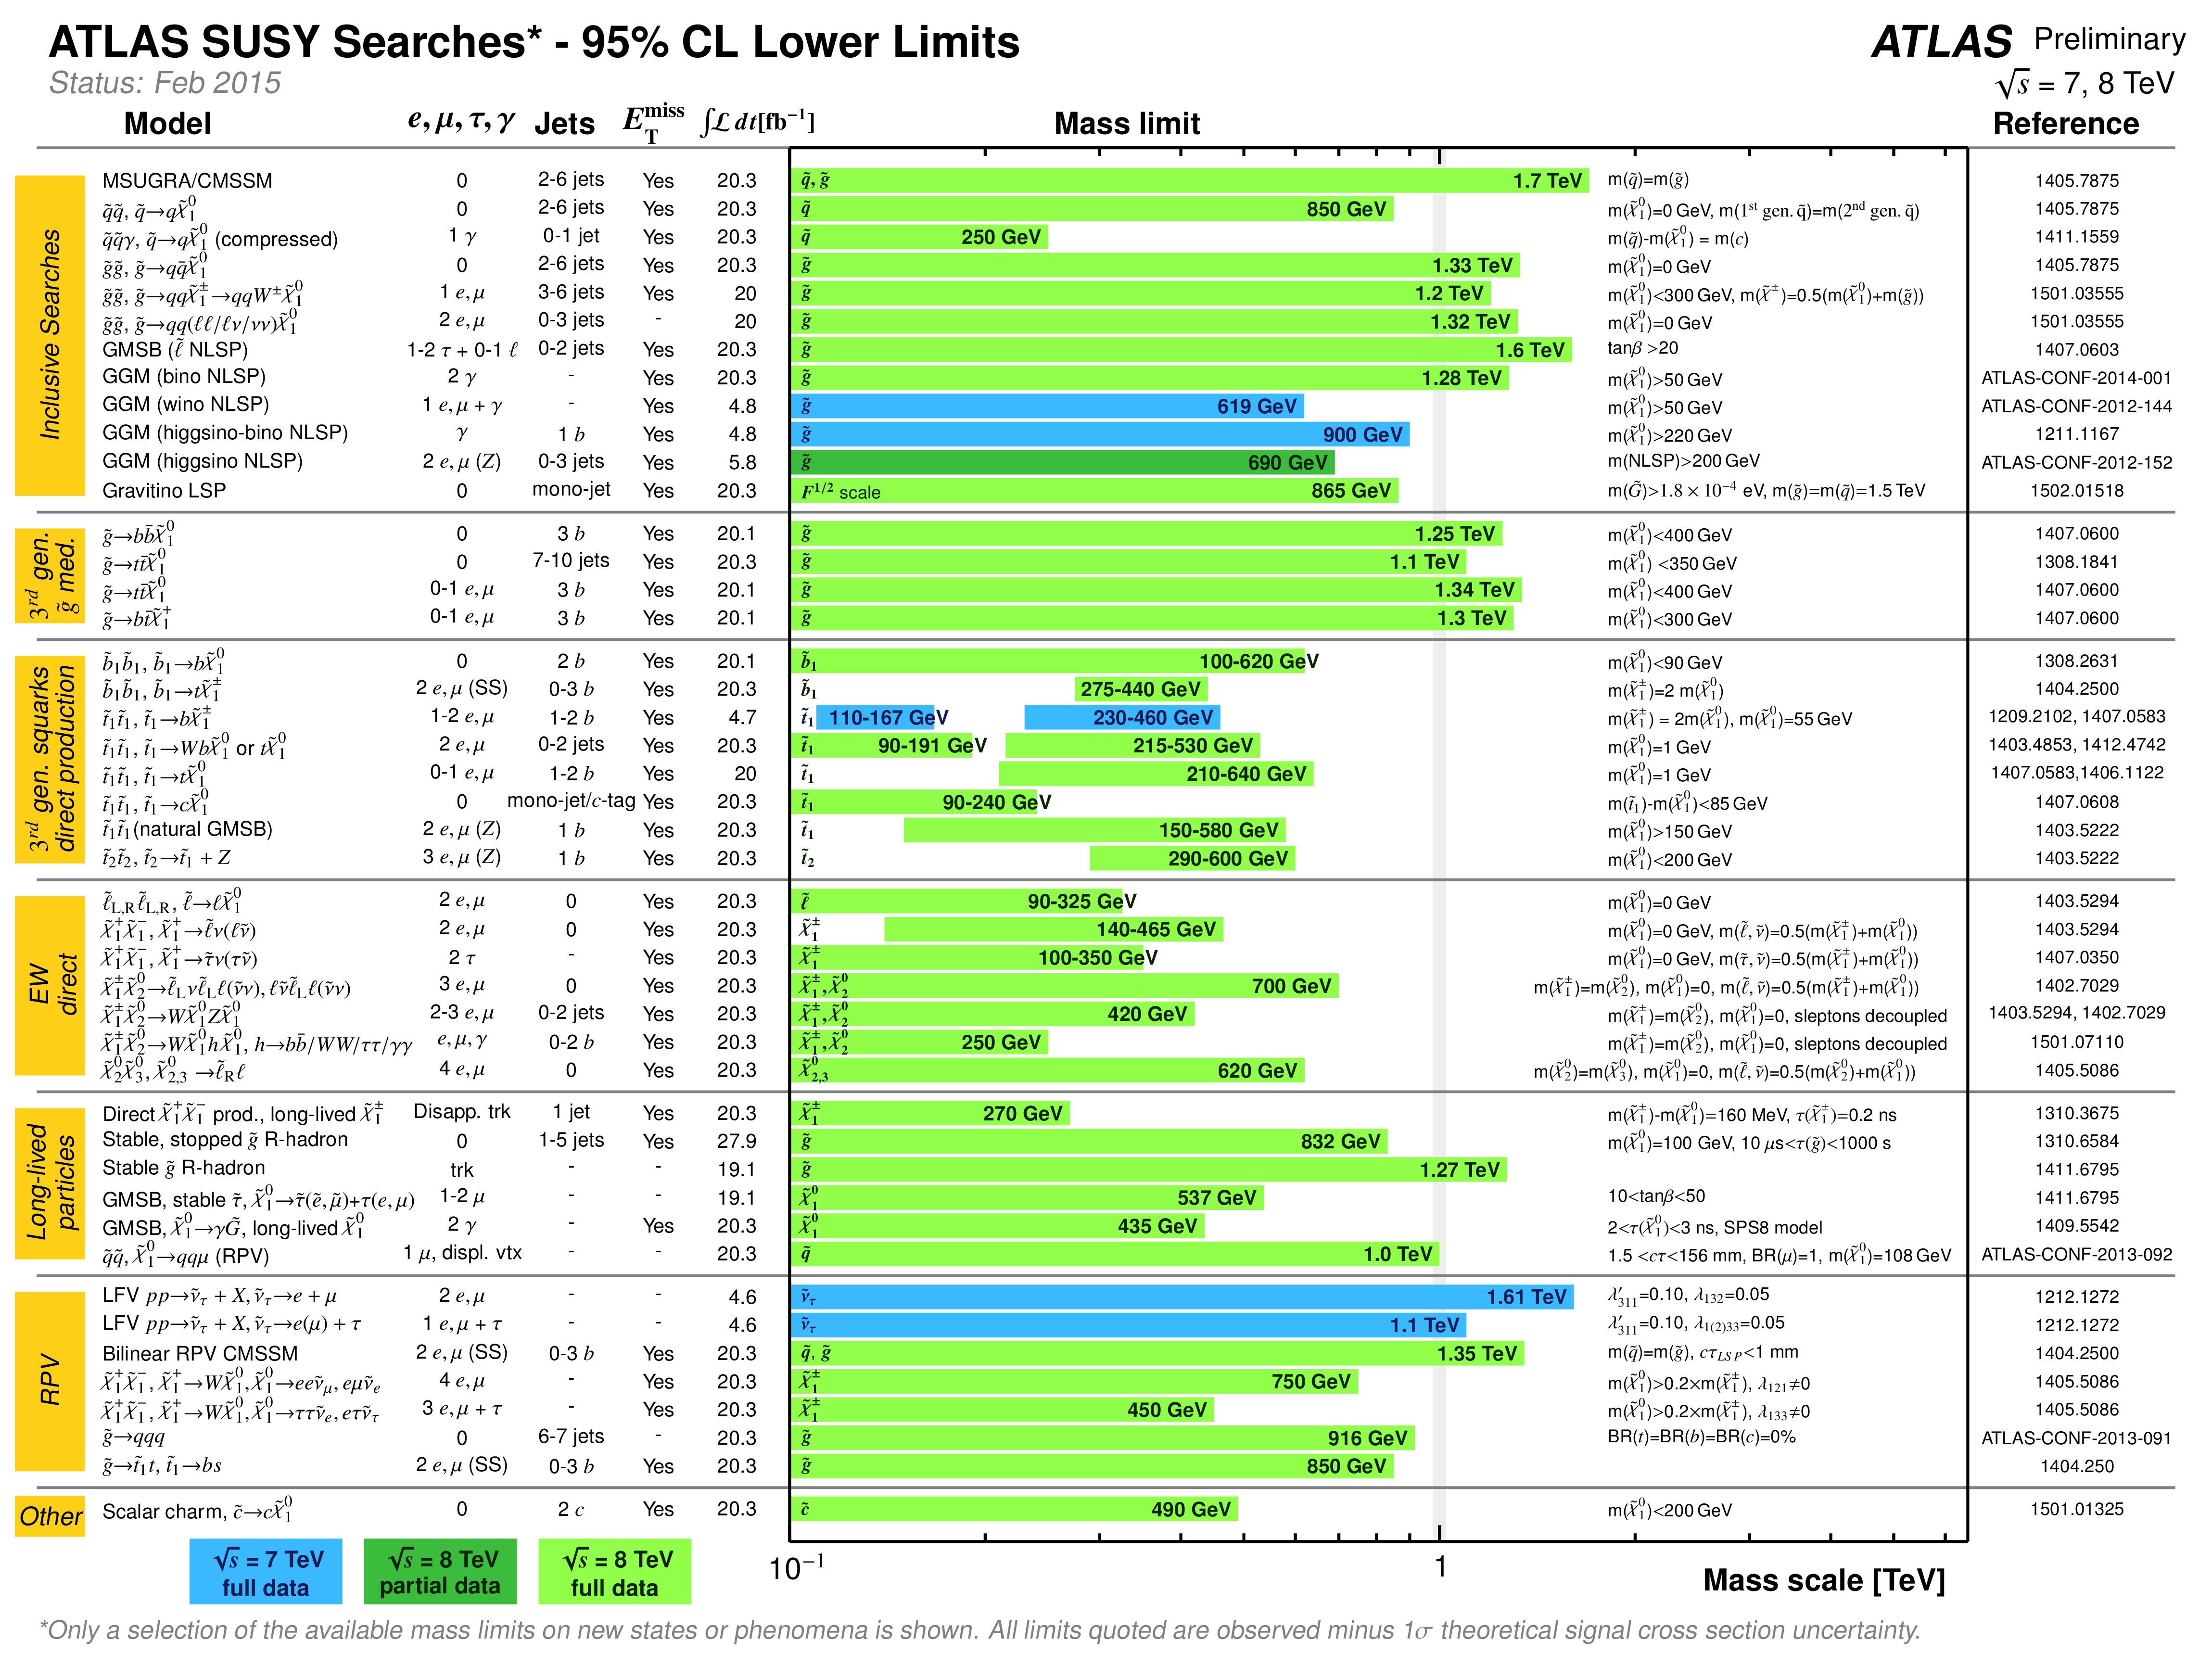
\includegraphics[width=1\textwidth]{figures/susyintro/ATLAS_SUSY_Summary.png}
	\caption{Summary of ATLAS SUSY limits per feb.\ 2015. }
	\label{fig:higgspot}
\end{figure}

\begin{figure}[hbt]
	\centering
	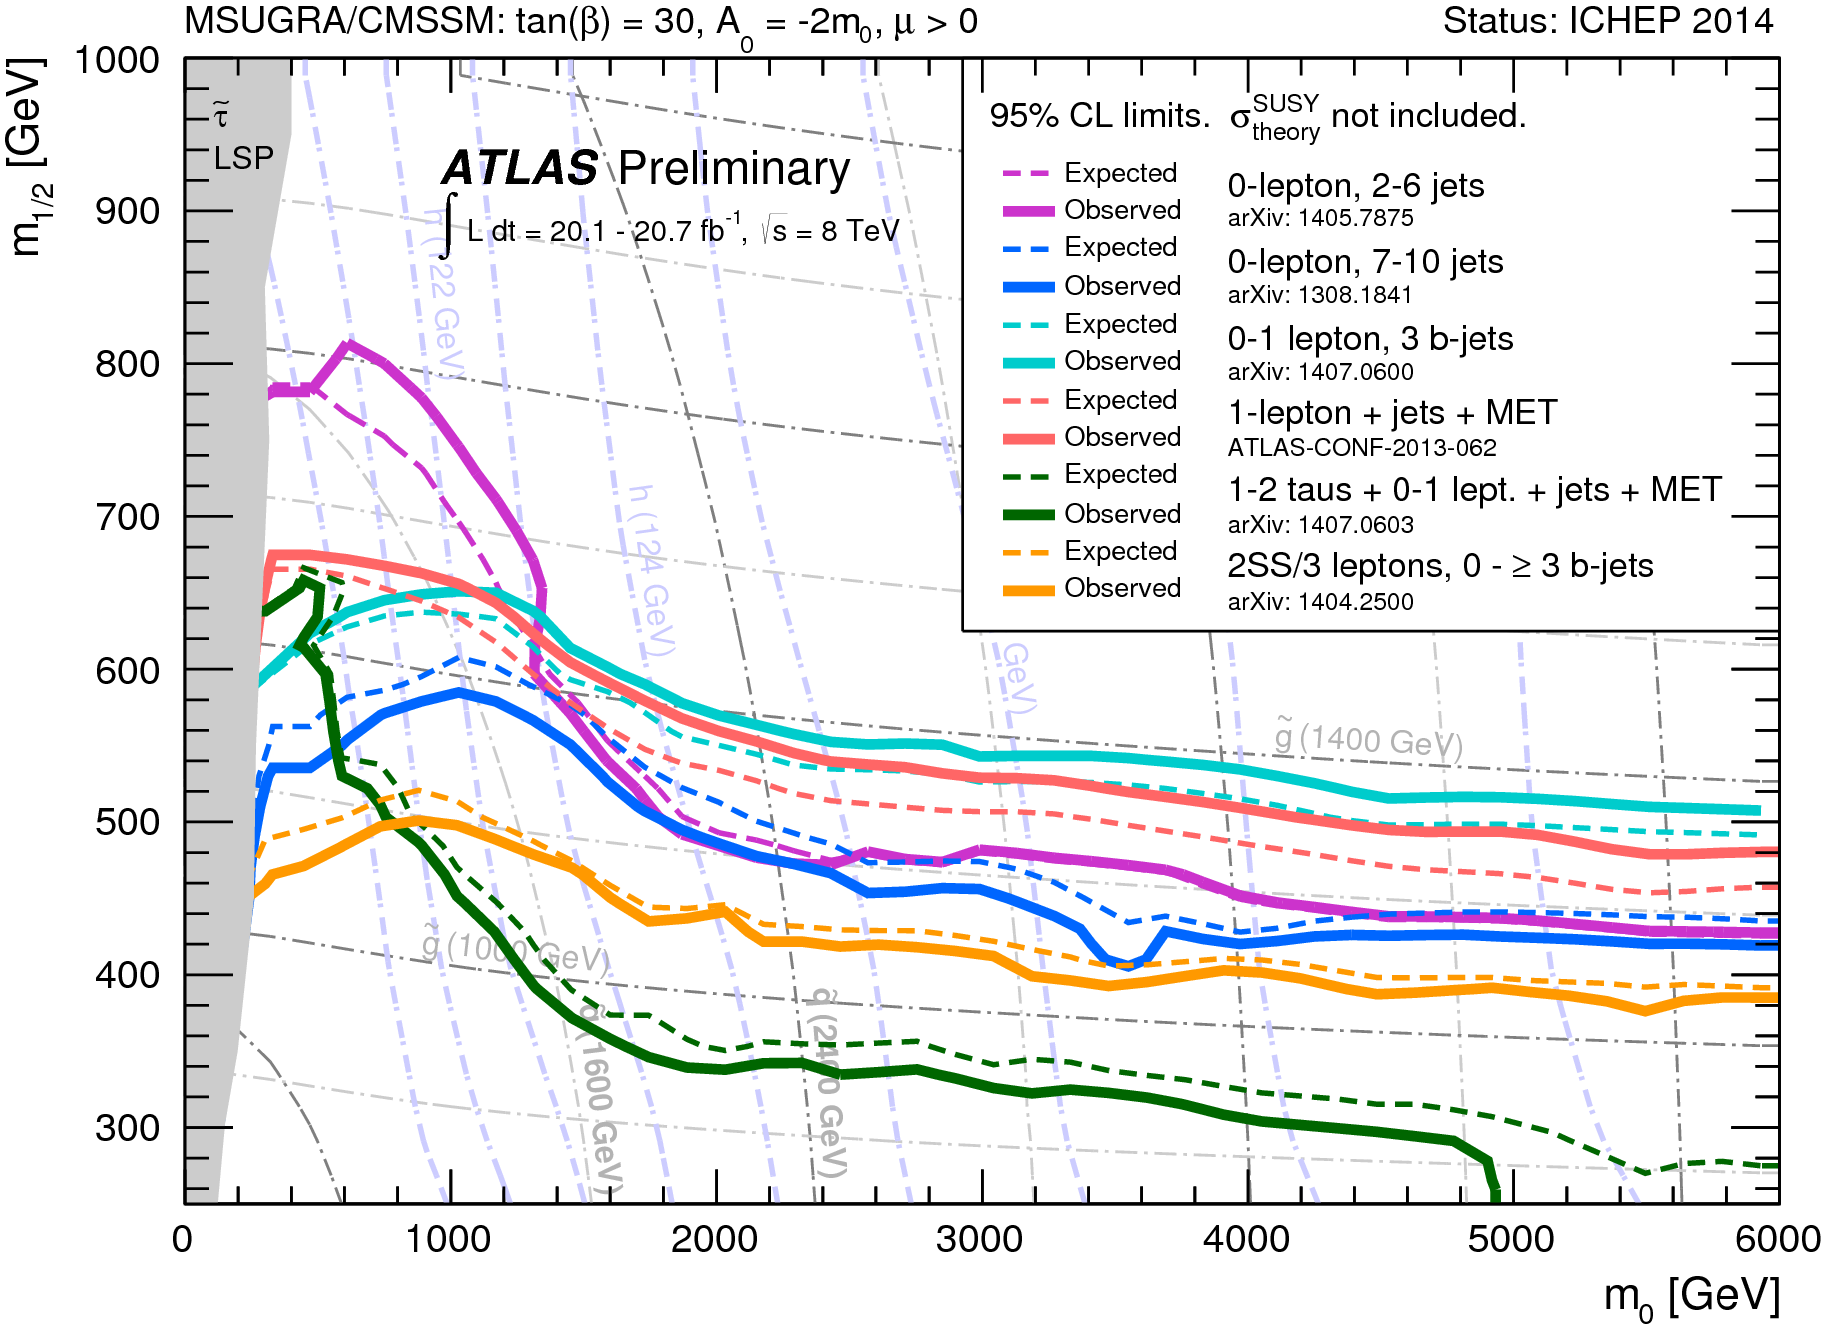
\includegraphics[width=0.9\textwidth]{figures/susyintro/ATLAS_SUSY_MSUGRA.png}
	\caption{mSUGRA/CMSSM limits from ATLAS per feb.\ 2015. }
	\label{fig:higgspot}
\end{figure}